\documentclass[a4paper]{article}

\usepackage{INTERSPEECH2019}
\usepackage{cite}
\usepackage{tablefootnote}
\usepackage{color}
\usepackage{pifont}
\usepackage{footnote}
\makesavenoteenv{tabular}

\usepackage{soul}

\def\X#1{%
        % #1%
        % \textcircled{#1}%
        \raisebox{.9pt}{\textcircled{\raisebox{-.9pt}{#1}}}%
        % \ding{\numexpr171+#1\relax}%
}
\newcommand{\quotes}[1]{``#1''}
\setlength{\intextsep}{7pt plus 0pt minus 3pt} %distance between floats on the top or the bottom and the text
\setlength{\textfloatsep}{7pt plus 0pt minus 4pt}%distance between two floats
\setlength{\floatsep}{7pt plus 0pt minus 2pt}%distance
\title{Improving Unsupervised Subword Modeling Via Disentangled Speech Representation Learning and Transformation}
\name{Siyuan Feng, Tan Lee}%The maximum number of authors in the author list is twenty. If the number of contributing authors is more than twenty, they should be listed in a footnote or in acknowledgement section, as appropriate.
\address{
  Department of Electronic Engineering, The Chinese University of Hong Kong, Hong Kong}
\email{siyuanfeng@link.cuhk.edu.hk, tanlee@ee.cuhk.edu.hk}

\begin{document}
% \ninept
\maketitle
% 
\begin{abstract}
This study tackles unsupervised subword modeling in the zero-resource scenario, learning frame-level speech representation that is phonetic discriminative and speaker-invariant, using only untranscribed speech for target languages. Frame label acquisition is an essential step in solving this problem. High quality frame labels  should be in good consistency with golden transcriptions and robust to speaker variation. We propose to improve frame label acquisition in our previously adopted deep neural network-bottleneck feature (DNN-BNF) architecture by applying the factorized hierarchical variational autoencoder (FHVAE). FHVAEs learn to disentangle linguistic content and speaker identity information encoded in speech. By discarding or unifying speaker information, speaker-invariant features are learned and fed as inputs to DPGMM frame labeling and DNN-BNF training. Experiments conducted on ZeroSpeech 2017 show that our proposed approaches achieve $2.4\%$ and $0.6\%$ absolute ABX error rate reduction in across- and within-speaker conditions, comparing to the baseline DNN-BNF system without applying FHVAEs.
% in across- and within-speaker conditions respectively. 
Our proposed approaches significantly outperform vocal tract length normalization in improving frame labels and subword modeling.
% Without requiring any out-of-domain data, our proposed approaches are able to

% achieve $77\%$ performance improvement 
% compensate for $77\%$ performance gap 
% Our previous attempt exploited out-of-domain resources in deep neural network-bottleneck feature (DNN-BNF) modeling
\end{abstract}
\noindent\textbf{Index Terms}: unsupervised subword modeling, disentangled representation, speaker-invariant feature, zero resource

\section{Introduction}
% With large amounts of speech and language resources 
Recent years have witnessed a huge success in applying deep learning  models in acoustic and language modeling for automatic speech recognition (ASR). 
% Typically, t
Training  deep neural network (DNN) acoustic models  requires large amounts of transcribed speech data. 
% This leads to the fact that high-performance ASR systems are only available for major languages. 
For many languages in the world, for which very little or no transcribed speech is available, conventional supervised acoustic modeling techniques cannot be  directly applied.

Unsupervised acoustic modeling (UAM) aims at discovering and modeling acoustic units  of an unknown language at subword or word level, assuming only untranscribed speech data are available.
UAM is a challenging problem with significant practical impact in speech  as well as linguistics and cognitive science communities. It has been studied in applications  such as ASR for low-resource languages \cite{I3EWang}, language identification \cite{li2007vector} and query-by-example spoken term detection \cite{Chen+2016}. This problem is also relevant to
% Solving this problem may also assist in
% It may also assist 
endangered language protection \cite{jansen2013summary} and  understanding infants' language acquisition mechanism \cite{dupoux2016cognitive}. 

Over the recent past, Zero Resource Speech Challenges (ZeroSpeech) 2015 \cite{versteegh2015zero} and 2017 \cite{dunbar2017zero} were organized to focus on unsupervised speech modeling.
% , focusing on unsupervised speech modeling, have attracted many researchers. 
ZeroSpeech 2017 Track one, named unsupervised subword modeling,  was formulated as an unsupervised feature representation learning problem, i.e., how to learn frame-level speech features that are discriminative to subword units and robust to linguistically-irrelevant variations such as speaker identity. 
The present study addresses this problem.
% {\color{blue}why repr. learning is an important issue in Un. speech modeling.}
% {\color{blue} 
It is a fundamental problem in unsupervised speech modeling.
% form the basis of several applications, such as keyword spotting, a good starting point for robust document retrieval. 
Speech simultaneously encodes linguistic-relevant information e.g. subword units and linguistic-irrelevant information e.g. speaker variation that are not easily separable. In supervised acoustic  modeling, golden transcription can be relied on to ensure the robustness of the learned subword units. In the unsupervised scenario, linguistic knowledge e.g. subword units and word patterns can only be  inferred from speech features. This makes feature representation learning important in unsupervised speech modeling. In the literature, there have been works showing that representation learning is beneficial to downstream applications such as spoken query retrieval \cite{chen2017multitask}.
% }
% Researchers proposed various approaches for comparison \cite{heck2017feature,chen2017multilingual,yuan2017extracting,ansari2017deep,shibata2017composite,Feng2018exploiting}. Cluster posteriorgram \cite{chen2015parallel,heck2017feature,ansari2017unsupervised},  DNN bottleneck features (BNFs) \cite{chen2017multilingual,yuan2017extracting},  autoencoders (AEs) and their variants \cite{renshaw2015comparison,ansari2017deep} are among the widely adopted  approaches. There are also works  assuming transcribed speech data for  out-of-domain languages  available, and building systems in a transfer learning manner \cite{shibata2017composite,Feng2018exploiting}. 
% unsupervised feature representation learning, and follows the purely unsupervised condition. 

In our previous attempt to ZeroSpeech 2017  \cite{Feng2018exploiting}, a  DNN was trained with   zero-resource speech data to generate bottleneck features (BNFs) as the learned feature representation. Frame labels for supervised DNN training were obtained through Dirichlet process Gaussian mixture model (DPGMM) based frame clustering. This framework is similar to \cite{chen2017multilingual}.
% The absence of transcription for the training data drove us to perform frame clustering and labeling, so as to enable supervised DNN-BNF training. 
By employing  out-of-domain transcribed speech data for speaker adapted feature learning and DNN frame labeling, the results in \cite{Feng2018exploiting} significantly outperform  \cite{chen2017multilingual} in which out-of-domain data were not employed. 
This improvement is mainly attributed to the advancement of frame label acquisition.   
% {\color{red} what's meant by good label? why are they critical?}
% {\color{blue}
Ideally, the learned  frame labels should have a full coverage of linguistically-defined phonemes. They should be  in good consistency with golden transcription and  robust to speaker variation. The quality of frame labels has a significant influence on the performance of subword modeling \cite{heck2017feature}.
% Frame labeling is an essential step in unsupervised subword modeling.  
% have a good coverage of ground-truth phonemes. In perfect consistency with linguistically-defined subword units.
% }
% DPGMM clustering towards speaker adapted features was found to generate better labels than towards unadapted features. 
% Similar properties were also observed in
Many prior works found out that DPGMM clustering towards speaker adapted features could generate better labels than that towards unadapted features \cite{HeckSN16,heck2017feature,chen2017multilingual}. In \cite{chen2017multilingual}, the authors compared MFCC features with and without vocal tract length normalization (VTLN) for clustering. 
In \cite{heck2017feature}, MFCCs were first clustered to generate initial tokenization, with which  linear transforms such as LDA, MLLT and fMLLR  were estimated. The fMLLRs are clustered again to generate final frame labels. This work achieved the best performance in ZeroSpeech 2017. One issue is that DPGMM frame clustering requires high computational costs. Typically, clustering towards $40$-hour speech data for $100$ iterations using $32$ CPU cores takes $25$ hours. This makes the system in \cite{heck2017feature} much heavier than  \cite{chen2017multilingual,Feng2018exploiting}.

In the strict zero-resource scenario, out-of-domain speech and language resources are unavailable. 
This paper proposes to improve DPGMM  frame labeling using only in-domain untranscribed speech data, and refrain from performing multiple-pass clustering processes.
% In this paper, we propose to improve DPGMM based frame labeling with limited speech resources and 
% we propose to improve our DNN-BNF based unsupervised subword modeling framework \cite{Feng2018exploiting} by performing speaker-invariant feature learning using 
% perform speaker-invariant feature learning by employing 
% the factorized hierarchical variational AE (FHVAE) model \cite{hsu2017nips}.
% in our DNN-BNF framework \cite{Feng2018exploiting}. 
Specifically, the factorized hierarchical variational AE (FHVAE) model \cite{hsu2017nips} is used to disentangle linguistic content and speaker information in raw speech features in an unsupervised manner. By either discarding or unifying speaker information, speaker-invariant representation is learned and  used as the input to DPGMM clustering and DNN-BNF training. 
% This idea is motivated by the fact that
% {\color{blue}[not coherent?]FHVAE models learn to factorize sequence-level and segment-level   attributes into different latent variables.}
The FHVAE is an unsupervised generative model.
% , making it suitable for the zero-resource scenario.
% , which makes it suitable for the zero-resource scenario.
% It is feasible for disentangling linguistic content and speaker inforamtion
% Intuitively, speaker characteristics is relatively invariant in short time span, as compared to linguistic content such as subword units.  
%(too specific, too detailed) After FHVAE training, speech utterances can be represented by speaker-invariant latent segment-level variables, as nuisance speaker information is embedded mainly in sequence-level variables. Besides, by unifying  sequence-level variables of all utterances while keeping segment-level variables unchanged, one could obtain reconstructed speech with FHVAE decoder as if they were spoken by the same speaker. The linguistic content from original to reconstructed speech is not changed.
% without changing linguistic content.
% FHVAE is an unsupervised generative model, which makes it suitable for the concerned zero-resource scenario. 
It was originally proposed for domain adaptation problems with applications to noise robust ASR \cite{hsu2018extracting}, distant conversational ASR \cite{hsu2018unsup},  and later applied to dialect identification \cite{shon2018unsup}. To the best of our knowledge, the use of FHVAEs in unsupervised subword modeling  has never been studied before. 

\section{Speaker-invariant feature learning by FHVAE}
% Raw spectral features contain abundant speaker identity information, which is harmful for  our concerned UAM problem. 
% To suppress speaker variation in speech and learn phonetic discriminative representation for UAM, a possible way is to disentangle linguistic content and speaker characteristics. Intuitively, 
% and only retain the former part.  
Speaker characteristics tends to have a smaller amount of variation than linguistic content within a speech  utterance, while linguistic content tends to have similar amounts of variation within and across utterances. The FHVAE model \cite{hsu2017nips}, which learns to factorize sequence-level and segment-level   attributes of sequential data into different latent variables, 
is applied in this work to disentangle linguistic content and speaker characteristics.
% factorize sequence-level attributes, i.e. speaker identity, and segment-level attributes, i.e. linguistic content, into different latent variables.
% to be reflected in speech representation at utterance level, while linguistic content tends to be reflected at segment level.
% is consistent within each utterance, while linguistic content tends to vary much faster and 

% This section gives a brief overview of the FHVAE model, and discuss how it can be applied to disentangle linguistic content and speaker identity information.
% Speech encodes multiple types of information such as linguistic content and speaker identity. 
% including linguistic content such as subword units and speaker identity. 
% In the concerned unsupervised feature representation learning task, speaker identity is a nuisance factor, 
\subsection{FHVAE model}
FHVAEs formulate the generation process of sequential data by imposing sequence-dependent priors and sequence-independent priors to different sets of variables. 
Following notations and terminologies in \cite{hsu2017nips}, 
% The graphical model of FHVAEs is shown in Figure {\color{blue}X}. 
let $\bm{z_1}$ and $\bm{z_2}$ denote latent segment variable and latent sequence variable, respectively. $\bm{\mu_2}$ is sequence-dependent prior, named as \emph{s-vector}. $\theta$ and $\phi$ denote the parameters of generation and inference models of FHVAEs.
Let $\mathcal{D}=\{\bm{X^{i}}\}_{i=1}^{M}$ denote a speech dataset with $M$ sequences. 
% $\bm{X_i}$ is a sequence of speech features formed by concatenating all speech utterances belonging to speaker $i$. 
Each $\bm{X^i}$ contains $N^i$ speech segments $\{\bm{x^{(i,n)}}\}^{N^i}_{n=1}$, where $\bm{x^{(i,n)}}$ is composed of fixed-length consecutive 
% $\bm{x_i^n}\in \mathbb{R}^{d\times l}$ is composed of $l$ consecutive
frames. The FHVAE model generates a sequence $\bm{X}$ from a random process as follows: (1) $\bm{\mu_2 }$ is drawn from a prior distribution $p_{\theta}(\bm{\mu_2})=\mathcal{N} (\bm{0},\sigma^2_{\mu_2} \bm{I})$; (2) $\bm{z_1 ^{n}} $ and $\bm{z_2^{n}} $ are drawn from $p_{\theta}(\bm{z_1 ^{n}})=\mathcal{N} (\bm{0}, {\sigma^2_{z_1}} \bm{I})$ and  $p_{\theta}(\bm{z_2 ^{n}| \bm{\mu_2}})=\mathcal{N}(\bm{\mu_2}, {\sigma^2_{z_2}} \bm{I} )$ respectively; (3) Speech segment $\bm{x^{n}}$ is drawn from $p_{\theta}(\bm{x^{n}}|\bm{z_1 ^{n}, \bm{z_2^{n}}})=\mathcal{N}(f_{\mu_x} (\bm{z_1 ^{n}}, \bm{z_2^{n}}), diag(f_{\sigma^2_x} (\bm{z_1 ^{n}}, \bm{z_2^{n}}))$. Here $\mathcal{N}$ denotes standard normal distribution, $ f_{\mu_x} (\cdot, \cdot)$ and $ f_{\sigma^2_x} (\cdot, \cdot)$ are parameterized by DNNs.
The joint probability for $\bm{X}$ is formulated as,
\begin{equation}
    p_{\theta} (\bm{\mu_2})\prod_{n=1}^{N} p_{\theta} (\bm{z_1^n}) p_{\theta} (\bm{z_2^{n}}|\bm{\mu_2})p_{\theta} (\bm{x^n}|\bm{z_1 ^{n}, \bm{z_2^{n}}}).
\end{equation}

Similar to VAE models, FHVAEs introduce an inference model $q_{\phi}$
% $q_{\phi} (\bm{Z_1}, \bm{Z_2}, \bm{\mu_2}| \bm{X})$ 
to approximate the intractable  true posterior as,
\begin{equation}
   q_{\phi} (\bm{\mu_2})\prod_{n=1}^{N}q_{\phi} (\bm{z_2^n}| \bm{x^n}) q_{\phi}(\bm{z_1^n}|\bm{x^n}, \bm{z_2^n}).
   \label{eqt:inference}
\end{equation}
Here  $q_{\phi} (\bm{\mu_2}), q_{\phi} (\bm{z_2^n}| \bm{x^n})$ and $q_{\phi}(\bm{z_1^n}|\bm{x^n}, \bm{z_2^n})$ are all diagonal Gaussian distributions. The mean and variance values of $q_{\phi} (\bm{z_2^n}| \bm{x^n})$ and $q_{\phi}(\bm{z_1^n}|\bm{x^n}, \bm{z_2^n})$ are parameterized by two DNNs. For $q_{\phi} (\bm{\mu_2})$, during FHVAE training, a trainable lookup table containing posterior mean of $\bm{\mu_2}$ for each sequence is updated.
% and the table is treated as trainable parameters. 
During testing, maximum a posteriori (MAP) estimation is used to infer  $\bm{\mu_2}$ of unseen test sequences with details described in \cite{hsu2017nips}.

FHVAEs optimize discriminative segmental variational lower bound $\mathcal{L} (\theta, \phi; \bm{x^{(i,n)}})$ defined as,
\begin{align*}
&\mathbb{E}_{q_{\phi} (\bm{z_1^{(i,n)}},\bm{z_2^{(i,n)}}|\bm{x^{(i,n)}} )} [\log p_{\theta} (\bm{x^{(i,n)}}|\bm{z_1^{(i,n)}}, \bm{z_2^{(i,n)}})] -\\
& \mathbb{E}_{q_{\phi}(\bm{z_2^{(i,n)}} |\bm{x^{(i,n)}} )} [\mathrm{KL} (q_{\phi} (\bm{z_1^{(i,n)}}|\bm{x^{(i,n)}}, \bm{z_2^{(i,n)}}))||p_{\theta} (\bm{z_1^{(i,n)}})]\\
&-\mathrm{KL} (q_{\phi}(\bm{z_2 ^{(i,n)}}|\bm{x^{(i,n)}})|| p_{\theta}(\bm{z_2 ^{(i,n)}}| \bm{\tilde{\mu}_2^i})) \\
&+\frac{1}{N^i}\log p_{\theta} (\bm{\tilde{\mu}_2^i}) + \alpha \log p(i| \bm{z_2^{(i,n)}}),
\end{align*}
where $i$ is sequence index, $\bm{\tilde{\mu}_2^{i}}$ denotes posterior mean of $\bm{\mu_2}$ for the $i$-th sequence, $\alpha$ denotes discriminative weight. The discriminative objective $\log p(i| \bm{z_2^{(i,n)}}) $ is defined as $\log p_{\theta} (\bm{z_2^{(i,n)}}| \bm{\tilde{\mu}_2^i})-\log \sum_{j=1}^{M}p_{\theta} (\bm{z_2^{(j,n)}}| \bm{\tilde{\mu}_2^j})$.

% The choice of $l$ should reflect the texture of linguistic content, i.e. subword units in this study. 
% a subset  corresponding to speaker $i$. Assume speech utterances of each
After FHVAE training, $\bm{z_2}$ encodes factors that are relatively consistent within a sequence.
% latent sequence variable $\bm{z_2}$ is expected to encode speaker identity information in original speech representation, as 
The discriminative objective ensures that $\bm{z_2}$ captures sequence-dependent information. $\bm{z_1}$ encodes residual factors that are sequence-independent.
% Speech utterances of the same speaker are concatenated to a long sequence s.t. each speaker TO a sequence
% It is an extension to VAEs.

% $z_1, z_2, \mu_2$; lower bound, discriminative loss; dnn architecture is lstm; input is fixed-length speech segments, a segment mapped to a latent variable
\subsection{Extracting speaker-invariant features by FHVAE}
\label{subsec:spk_inv_feat}
% 1 intro of FHVAE
% 2 state two types of speaker-invariant features, z1 and unifying mu2.
% that is relatively consistent within a sequence. 
In order to apply the FHVAE model to learn speaker-invariant features, 
% The FHVAE model is applied to disentangle linguistic content and speaker characteristics encoded in speech. To this end, 
training utterances of the same speaker are concatenated into a single sequence.
By this means, 
% Suppose in a speech dataset $\mathcal{D}$ for FHVAE training, utterances belonging to the same speaker are concatenated to a single sequence, then 
$\bm{z_2}$ is expected to encode speaker identity information and  carry little phonetic information. $\bm{z_1}$ is expected to encode residual information, i.e. linguistic content, and  invariant to speaker identity. 
% Based on the disentangled speech representation
This work considers two methods to obtain speaker-invariant feature representation based on a trained FHVAE. The first method is straightforward to treat 
% \subsubsection{d}
latent segment variables $\{\bm{z_1^{(i,n)}}\}$ as the desired  feature representation. 
% {\color{blue}[move to exp section?]Since our concerned UAM problem targets  frame-level representation learning, during latent variable inference  the input segments are shifted  by one frame. }
% while $\bm{z_1^n}$ is inferred from speech segment $\bm{x^n}$.
% According to Equation (\ref{eqt:inference}), the inference of $\bm{z_1^n}$ depends on a speech segment. 

In the second method, the FHVAE model reconstructs speech features of all utterances based on a unified s-vector. The reconstructed features are the desired representation.
% s-vectors $\{\bm{\mu_2^{i}}\}$ of all the speech sequences are modified to the same value. 
Specifically, a representative speaker with his/her s-vector (denoted as $\bm{\mu_2^*}$) is chosen from the dataset. Next, for each speech segment $\bm{x^{(i,n)}}$ of an arbitrary speaker $i$, its corresponding latent sequence variable $\bm{z_2^{(i,n)}}$ is transformed to $\bm{\hat{z}_2^{(i,n)}}=\bm{z_2^{(i,n)}}-\bm{\mu_2^i}+\bm{\mu_2^*}$, where $\bm{\mu_2^{i}}$ denotes s-vector of speaker $i$. 
Finally the decoder network of the FHVAE model reconstructs segment $\bm{\hat{x}^{(i,n)}}$ conditioned on $\bm{z_1^{(i,n)}}$ and $ \bm{\hat{z}_2^{(i,n)}}$. This method is named as \emph{s-vector unification} in the present work.
% The reconstructed features $\{\bm{\hat{x}^{(i,n)}}\}$ are our desired speaker-invariant representation. 
Compared to original features,  reconstructed features  are expected to keep the  linguistic content unchanged and capture speaker characteristics corresponding to the representative speaker. In other words, the speech synthesized by $\{\bm{\hat{x}^{(i,n)}}\}$ would ideally sound as if they were all spoken by the representative speaker. 
% unifying the speaker characteristics to the representative speaker.
% Specifically, ... find a representative speaker, its s-vector denoted as..

% segment variable $\bm{z_1}$ is expected to  encode linguistic content speech utterances can be represented by speaker-invariant latent segment-level variables, as nuisance speaker information is embedded mainly in sequence-level variables. 
% Besides, by unifying  sequence-level variables of all utterances while keeping segment-level variables unchanged, one could obtain reconstructed speech with FHVAE decoder as if they were spoken by the same speaker. The linguistic content from original to reconstructed speech is not changed.
\section{Unsupervised subword modeling with speaker-invariant features}

\subsection{DNN-BNF architecture}
A DNN-BNF architecture  \cite{chen2017multilingual,Feng2018exploiting} is adopted to perform  phonetic discriminative training of untranscribed speech data and generate BNFs for subword modeling. 
% In the literature, input features for DNN-BNF were MFCCs+VTLN  \cite{chen2017multilingual} or fMLLRs estimated by a pre-trained out-of-domain ASR \cite{Feng2018exploiting}.
% In this study, speaker-invariant features obtained by an FHVAE model are used as inputs to the DNN-BNF architecture. 
In this  architecture, given untranscribed speech data of each target zero-resource language, Dirichlet process Gaussian mixture model (DPGMM) \cite{chang2013parallel} algorithm is applied to perform frame clustering towards speech features. After clustering, each frame is assigned with a cluster label. These frame labels  are regarded as pseudo phoneme alignments to support supervised DNN training. A multilingual DNN with a linear bottleneck layer is trained with frame alignments  of all the target languages simultaneously, using multi-task learning  \cite{caruana1998multitask}. After training, subword discriminative BNFs are extracted as the learned representation.

\subsection{DNN-BNF training with speaker-invariant features}
Speaker-invariant features learned by FHVAEs are applied  in the DNN-BNF architecture 
% can be made 
% is twofold. 
in two aspects.
As can be seen in Figure \ref{fig:framework}, during DPGMM-based frame clustering,  input features to DPGMM are reconstructed MFCCs $\{\bm{\hat{x}}\}$ generated by the FHVAE decoder network using the s-vector unification method described in Section 
% with a pre-defined  s-vector as mentioned in Section 
\ref{subsec:spk_inv_feat}. Compared to original MFCCs, FHVAE reconstructed MFCCs  carry speaker information that is more consistent across utterances spoken by different speakers. With the reconstructed features as inputs, DPGMM clustering is expected to  generate better phoneme-like labels and less affected by speaker variation. 
% The selection of representative s-vector $\bm{\mu_2^*}$ is flexible.

During  DNN-BNF model training,  FHVAE-based speaker-invariant features are  fed as  inputs to the DNN. As seen in Figure \ref{fig:framework}, in this study we consider two feature types, i.e.  reconstructed MFCCs with s-vector unification $\{\bm{\hat{x}}\}$  and latent segment variables $\{\bm{z_1}\}$, as DNN inputs. Their effectiveness is evaluated and compared in this study.  
% and evaluate their effectiveness.  
% , meanwhile keeping linguistic content unchanged.  
\begin{figure}[t]
    \centering
    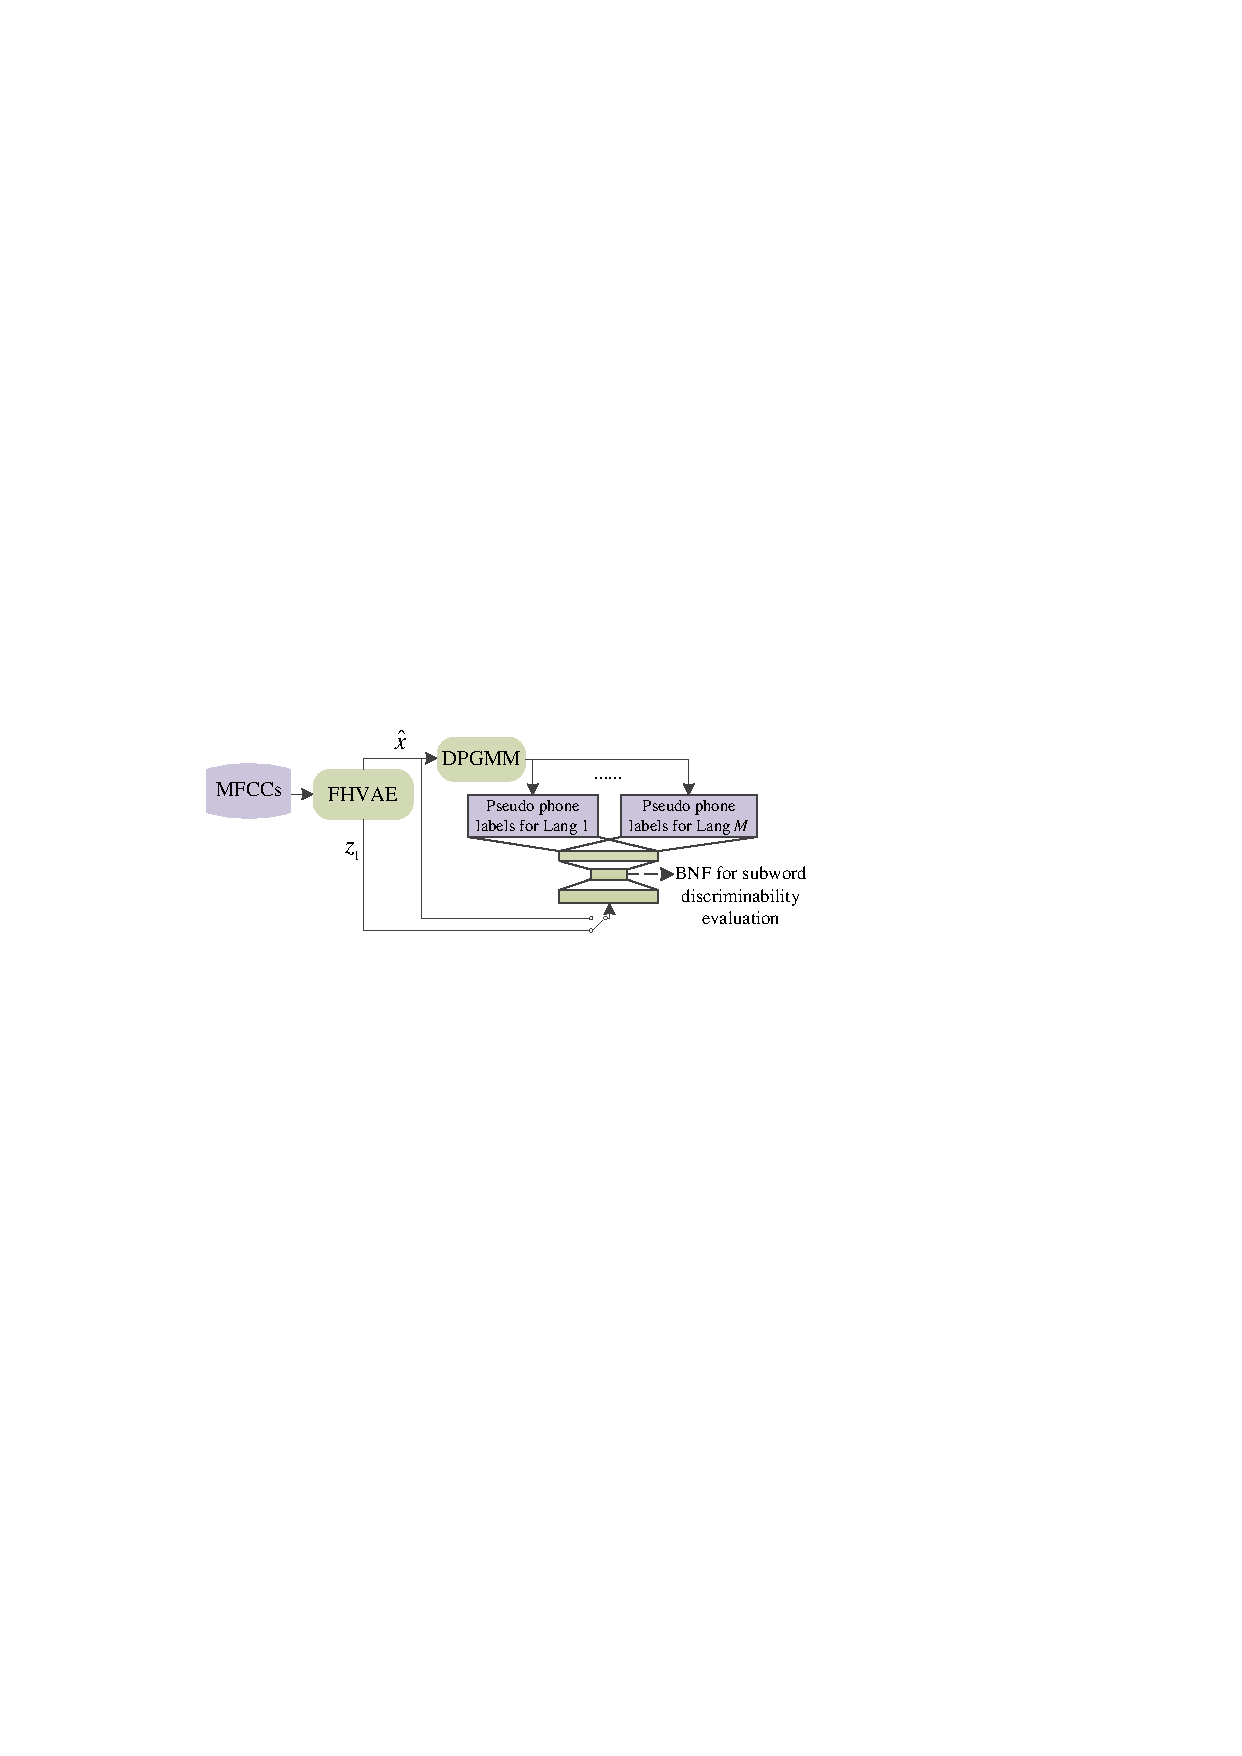
\includegraphics[width=0.9\linewidth]{framework.pdf}
    \caption{DNN-BNF architecture with FHVAE-based speaker-invariant features for subword discriminability task}
    \label{fig:framework}
\end{figure}
\section{Experimental setup}
\subsection{Dataset and evaluation metric}
Experiments are carried out with development data of ZeroSpeech 2017 Track one \cite{dunbar2017zero}.
% , \textit{unsupervised subword modeling} task \cite{dunbar2017zero}. 
The dataset consists of three languages, i.e., English, French and Mandarin. 
% Each language contains separate training and test sets of untranscribed speech. 
Speaker identity information is released only for train sets. Test sets are organized into subsets of differing utterance length (1s, 10s and 120s). Detailed information  is listed in Table \ref{tab:zr17_data}.
% \footnote{`speakers-R/-L' denotes speakers with rich/limited speech data.}. 
% In this Table, `speakers-R/-L' denotes speakers with rich/limited speech data.

\begin{table}[htbp]
\renewcommand\arraystretch{0.8}
\centering
\caption{Development data in ZeroSpeech 2017 Track one}
\resizebox{0.8 \linewidth}{!}{%
\begin{tabular}{lccc|c}      
% \hline      
\toprule
 & \multicolumn{3}{c|}{ Training} & Test \\
% \midrule
 & Duration  &\#speakers-R\tablefootnote{`speakers-R/-L' denotes speakers with rich/limited speech data.} &\#speakers-L  & Duration\\
% \hline
\midrule
English & $45$ hrs &$9$& $60$ & $27$ hrs\\
French & $24$ hrs &$10$& $18$ & $18$ hrs\\
Mandarin & $2.5$ hrs &$4$& $8$ & $25$ hrs\\
% Training hours:  & $19.3$ & $81.5$ & $105.3$ \\
% Test hours:& $0.6$ & $0.7$ & $5.9$ \\
% Basic acoustic unit:  & Phone & Phone & Initial-Final \\
% \#basic units (inc. sil):& $33$ & $87$ & $61$ \\
% \#tied CD-HMM states:& $2462$ & $3431$ & $2386$ \\ 
% Lexicon size:& $ $ & $ 133K$& $ $ \\
% $\#$ Phonemes: &$43$& $46$&$ 29$& $44$& $38$\\
% \hline
\bottomrule
\end{tabular}%
% \footnotetext{`speakers-R/-L' denotes speakers with rich/limited speech data}

}
\label{tab:zr17_data}
\end{table}

The evaluation metric is ABX subword discriminability. The ABX task is to decide whether $X$ belongs to $x$ or $y$ if $A$ belongs to $x$ and $B$ belongs to $y$, where $A$, $B$ and $X$ are three speech segments, $x$ and $y$ are two phonemes that differ in the central sound (e.g., \quotes{beg}-\quotes{bag}). 
Each pair of $A$ and $B$ are generated by the same speaker. 
ABX error rates for \textit{within-speaker} and \textit{across-speaker} are evaluated separately, depending on whether $X$ and $A(B)$ belong to the same speaker.
Dynamic time warping  and cosine distance are used to measure segment- and frame-level dissimilarity, respectively.
\subsection{FHVAE setup and parameter tuning}
% The FHVAE model with LSTM layers is used in this work. 
FHVAE model parameters are determined by referring to  \cite{hsu2018extracting}. The  encoder and decoder networks of FHVAE are both $2$-layer LSTMs with $256$ neurons per layer. The dimensions of  $\bm{z_1}$ and $\bm{z_2}$ are $32$. 
Training data of the three target languages are merged to train the FHVAE. 
Input features  are fixed-length speech segments randomly chosen from utterances. The determination of segment length $l$ is discussed in the next paragraph. Each frame is represented by a $13$-dimensional MFCC with cepstral mean normalization at speaker level. 
% During training, there is no frame overlapping between two adjacent segments. 
During the inference of reconstructed feature representation, input segments are shifted by $1$ frame. To match the length of extracted features with original MFCCs, the first and last frame are padded. 
% The loss function is negative discriminative segment variational lower bound with  discriminative weight $\alpha=10$.
Adam \cite{kingma2014adam} with $\beta_1=0.95$ and $\beta_2=0.999$  is used to train the FHVAE. A $10\%$ subset of training data is randomly selected for cross-validation.
The training process is terminated if the lower bound on the cross-validation set does not improve for $20$ epochs. Experiments are implemented in Tensorflow \cite{Abadi2016tensorflow}.

% Stopping criteria?
% The majority of FHVAE model parameters, set as suggested by \cite{hsu2018extracting} 
In our preliminary experiments, the ABX performance on $\bm{z_1}$ was found to be sensitive to the input segment length $l$. 
% This is in agreement with our expectation.
This could be explained as:  a too large  $l$ would reduce  $\bm{z_1}$'s capability in modeling linguistic content at  subword-level; 
% ambiguity of  $\bm{z_1}$ in terms of subword discriminability. 
a too small $l$ would limit the FHVAE in capturing sufficient temporal dependencies which are essential in modeling speech.  ABX error rates on $\bm{z_1}$ with different $l$s   are shown in Fig. \ref{fig:tune_len}. 
% The horizontal reference line denotes MFCC baseline \cite{dunbar2017zero}.  
The optimal value of $l$ is $10$. For the remaining experiments in this work, $l$ is fixed to $10$. In this setting, $\bm{z1}$ outperforms MFCC in both across- and within-speaker conditions.

\begin{figure}[t]
    \centering
    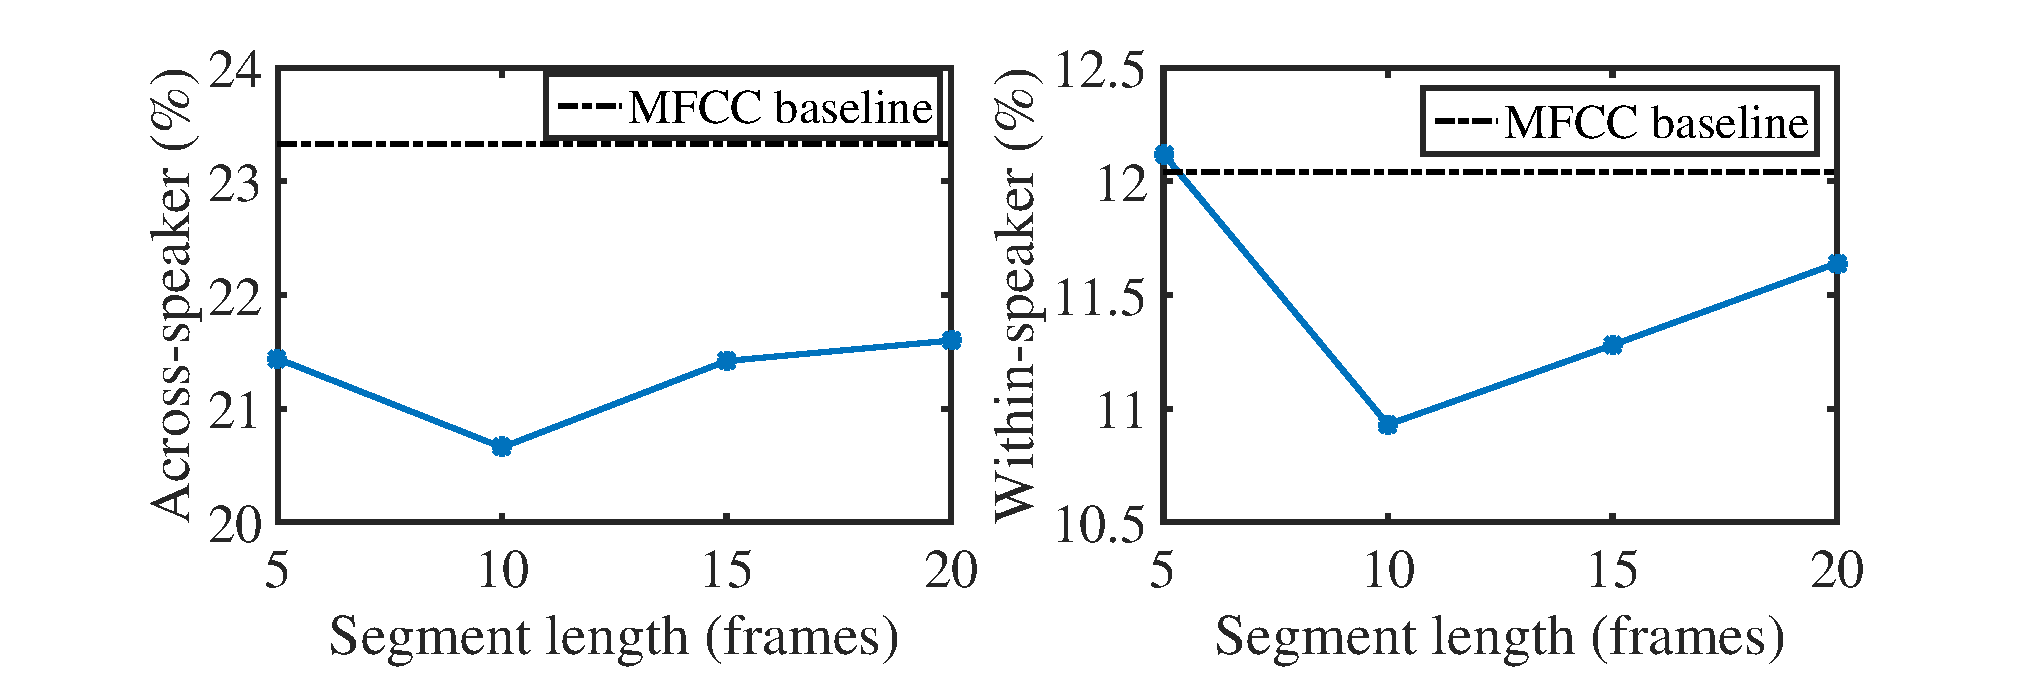
\includegraphics[width=0.9\linewidth]{tune_seg_len2_export_setup.eps}
    \caption{ABX error rates (\%) on  $\bm{z_1}$ with  different segment lengths and official MFCC baseline \cite{dunbar2017zero} (Avg. over languages).}
    \label{fig:tune_len}
\end{figure}


% \begin{table}[htbp]
% \renewcommand\arraystretch{0.8}
% \centering
% \caption{ABX error rates (\%) on  $\bm{z_1}$ with  different segment lengths and raw MFCCs. The results are averaged over three target languages.}
% \resizebox{0.75 \linewidth}{!}{%
% \begin{tabular}{c|cc}      
% % \hline      
% \toprule
%  Length (frames) &  Within-speaker & Across-speaker \\
% \midrule

% $5$ & $12.12$  & $21.44$  \\
% $10$ & $10.93$  & $20.66$ \\
% $20$ & $11.64$  & $21.60$ \\
% \midrule
% MFCCs \cite{dunbar2017zero} & $12.04$ &$23.33$ \\ 
% % Training hours:  & $19.3$ & $81.5$ & $105.3$ \\
% % Test hours:& $0.6$ & $0.7$ & $5.9$ \\
% % Basic acoustic unit:  & Phone & Phone & Initial-Final \\
% % \#basic units (inc. sil):& $33$ & $87$ & $61$ \\
% % \#tied CD-HMM states:& $2462$ & $3431$ & $2386$ \\ 
% % Lexicon size:& $ $ & $ 133K$& $ $ \\
% % $\#$ Phonemes: &$43$& $46$&$ 29$& $44$& $38$\\
% % \hline
% \bottomrule
% \end{tabular}%
% }
% \label{tab:tune_len}
% \end{table}
\begin{table*}[htbp]
\renewcommand\arraystretch{0.6}
\centering
\caption{ABX error rates ($\%$) on baseline and systems trained with FHVAE-based speaker-invariant features}
\resizebox{ 0.91\linewidth}{!}{%
\begin{tabular}{cll|ccc|ccc|ccc|c||ccc|ccc|ccc|c}      
% \hline      
\toprule
ID& && \multicolumn{10}{c||}{ Across-speaker} & \multicolumn{10}{c}{ Within-speaker} \\
\midrule
 & && \multicolumn{3}{c|}{ English} & \multicolumn{3}{c|}{ French} & \multicolumn{3}{c|}{Mandarin}& Avg.&\multicolumn{3}{c|}{ English} & \multicolumn{3}{c|}{ French} & \multicolumn{3}{c|}{Mandarin} & Avg.\\
&& & 1s & 10s & 120s & 1s & 10s & 120s & 1s & 10s & 120s && 1s & 10s & 120s & 1s & 10s & 120s & 1s & 10s & 120s\\ 
% \midrule
%  & Duration & \#speakers  & Duration\\
% \hline
\midrule
&\multicolumn{2}{l|}{Baseline} &$13.5$&$12.4$&$12.4$&$17.8$&$16.4$&$16.1$&$12.6$&$11.9$&$12.0$&$13.90$&$8.0$&$7.3$&$7.3$&$10.3$&$9.4$&$9.3$&$10.1$&$8.8$&$8.9$&$8.82$ \\
 & \multicolumn{2}{l|}{CA-Sup \cite{Feng2018exploiting} }&$10.9$&$9.5$&$8.9$&$15.2$&$13.0$&$12.0$&$10.5$&$8.9$&$8.2$&$10.79$&$7.4$&$6.9$&$6.3$&$9.6$&$9.0$&$8.1$&$9.8$&$8.8$&$8.1$&$8.22$ \\
\midrule
&\multicolumn{2}{l|}{MFCC \cite{chen2017multilingual}} &$13.7$&$12.1$&$12.0$&$17.6$&$15.6$&$14.8$&$12.3$&$10.8$&$10.7$& $13.29$&
 $8.5$&$7.3$&$7.2$&$11.1$&$9.5$&$9.4$&$10.5$&$8.5$&$8.4$&$8.93$
 \\
&\multicolumn{2}{l|}{MFCC+VTLN \cite{chen2017multilingual}}& $12.7$&$11.0$&$10.8$&$17.0$&$14.5$&$14.1$&$11.9$&$10.3$&$10.1$&$12.49$&$8.5$&$7.3$&$7.2$&$11.2$&$9.4$&$9.4$&$10.5$&$8.7$&$8.5$&$8.97$
 \\
 \midrule
\X1 &$\bm{z_1}$& Orig. &  $12.9$&$11.7$&$11.7$&$17.2$&$15.5$&$15.2$&$12.5$&$11.4$&$11.5$&$13.29$&$8.2$&$7.0$&$7.0$&$10.7$&$9.2$&$9.1$&$10.4$&$8.8$&$8.7$&$8.79$ \\

\X2 &$\bm{\tilde{x}}$& Orig.& $12.8$&$11.7$&$11.5$&$17.8$&$15.5$&$15.1$&$12.3$&$10.9$&$10.7$&$13.14$&$8.2$&$7.3$&$7.0$&$10.6$&$9.3$&$8.9$&$10.5$&$8.8$&$8.7$&$8.81$ \\

\X3& $\bm{z_1}$&$\bm{\hat{x}}$-s0107& $11.2$&$10.1$&$10.1$&$15.5$&$13.8$&$13.7$&$11.5$&$10.2$&$10.0$&$11.79$&$7.3$&$6.4$&$6.6$&$10.1$&$8.9$&$8.8$&$10.4$&$8.5$&$8.4$&$8.38$ \\

\X4& $\bm{\tilde{x}}$&$\bm{\hat{x}}$-s0107& $11.6$&$10.4$&$10.1$&$16.1$&$13.9$&$13.7$&$11.9$&$10.2$&$10.4$&$12.03$&$7.8$&$6.7$&$6.5$&$10.5$&$9.6$&$9.3$&$10.8$&$8.6$&$8.7$&$8.72$ \\

\X5& $\bm{z_1}$&$\bm{\hat{x}}$-s4018 & $11.0$&$9.8$&$9.8$&$14.9$&$13.4$&$13.0$&$11.4$&$10.1$&$10.0$&$\bm{11.49}$&$7.3$&$6.3$&$6.3$&$9.7$&$8.6$&$8.4$&$10.1$&$8.5$&$8.4$&$\bm{8.18}$ \\

\X6& $\bm{\tilde{x}}$&$\bm{\hat{x}}$-s4018& $11.3$&$10.0$&$9.8$&$15.7$&$13.6$&$13.3$&$11.8$&$10.0$&$10.4$&$11.77$&$7.8$&$6.5$&$6.5$&$10.1$&$9.1$&$8.8$&$10.6$&$8.7$&$8.7$&$8.53$ \\
\bottomrule
\end{tabular}%
}
\label{tab:results}
\end{table*}
\subsection{Selecting representative speaker for extracting reconstructed MFCCs}
%5, 10$ and $20$ are listed in Table 
The extraction of reconstructed MFCCs $\{\bm{\hat{x}}\}$ using s-vector unification assumes a pre-defined representative speaker. 
% In principle,  the selection  is flexible, which could be an arbitrary speaker in training data. 
In order to validate the generalization ability of our proposed s-vector unification method and measure its sensitivity to the gender of the representative speaker, $6$ English speakers \{s0107, s3020, s4018, s0019, s1724, s2544\}, $4$ French speakers \{M02R, M03R, F01R, F02R\} and $2$ Mandarin speakers \{A08, C04\} are randomly chosen from `speaker-R' sets of ZeroSpeech 2017 training data. 
% All the above speakers belong to `speakers-R'. 
The first half speakers  inside each language set  are male and the second half are female\footnote{Gender information is confirmed through listening.}. During the extraction of $\{\bm{\hat{x}}\}$, s-vectors  $\{\bm{\mu_2^i}\}$ of all three target languages' utterances are modified to the same $\bm{\mu_2^*}$  corresponding to one of the $12$ speakers mentioned above. The performance of  the $12$ groups of $\{\bm{\hat{x}}\}$ is evaluated by the ABX discriminability task.
% The ABX performance of $\{\bm{\hat{x}}\}$ extracted using  different representative speakers is conducted. 
% All of these $12$ speakers are chosen from those with rich per-speaker speech data.   

\label{subsec:repre_spk}
% {\color{blue}[where to describe the process of selecting 6 male and 6 female speakers randomly, and test the ABX performance of $\bm{\hat{x}}$ with each of these speakers ]}

\subsection{DNN-BNF setup}
% DPGMM clustering is implemented by an open-source tool \cite{chang2013parallel}. 
For the baseline system without using FHVAE-based speaker-invariant features,  input features  to DPGMM are  $39$-dimensional MFCCs+$\Delta$+$\Delta\Delta$. 
% Frames of each target language are clustered individually. 
The numbers of clustering iterations for English, French and Mandarin sets are $120,200$ and $3000$. After clustering, each frame is assigned with a label. A DNN-BNF model is trained with all three languages'  cepstral mean normalized MFCCs+$\Delta$+$\Delta\Delta$ and frame labels using  multi-task learning with equal task weights. 
% Task weights are the same for the three languages.
% with equal weights among the three language tasks.
% equally-weighted language tasks. 
% The input features are spliced with $\pm 5$. 
The dimensions of hidden layers are $\{1024\times5,40,1024\}$.
% , where the block-softmax layer dimensions depend on DPGMM cluster numbers, which are $1118, 1345$ and $596$ for English, French and Mandarin. 
After training, $40$-dimensional BNFs for test sets are extracted and evaluated by ABX subword discriminability. DPGMM is implemented using tools by \cite{chang2013parallel}. DNN-BNF training is implemented in Kaldi \cite{povey2011kaldi}.

For the systems employing FHVAE-based speaker-invariant features,  input features to DPGMM are reconstructed MFCCs $\{\bm{\hat{x}}\}$ with s-vector unification and further appended by $\Delta$+$\Delta\Delta$. 
The representative speaker is selected from the $12$ speakers mentioned in Section \ref{subsec:repre_spk}. 
% One of the $12$ speakers mentioned in Section \ref{subsec:repre_spk} is chosen as the representative speaker. 
The numbers of clustering iterations for the three languages are $80,80$ and $1400$. 
% Other DPGMM configurations are kept the same as in baseline.
DNN-BNFs are trained with either reconstructed MFCCs $\{\bm{\tilde{x}}\}$ or latent segment variables $\{\bm{z_1}\}$. The extraction of $\{\bm{\tilde{x}}\}$  is slightly different from $\{\bm{\hat{x}}\}$. During the  inference of $\{\bm{\tilde{x}}\}$ for ZeroSpeech training sets, s-vector unification is not applied;  during the inference for  test sets, s-vector unification is applied within every test subset with a subset-specific $\bm{\mu_2^*}$. 
The reason is that  DNN-BNFs  trained with $\{\bm{\tilde{x}}\}$ were found to outperform those trained with $\{\bm{\hat{x}}\}$.
% $\{\bm{\tilde{x}}\}$ were found to outperform 
% We found $\{\bm{\tilde{x}}\}$ outperform 
% $\{\bm{\hat{x}}\}$ in training the DNN-BNF model. 
The structure and loss function of DNN-BNFs keep the same as in the baseline system.

% DNN-BNF structure and training strategies.

% is adopted to perform DPGMM clustering towards speech frames of each target language.
% ,  ... DPGMM; inputs, original MFCCs or reconstructed MFCCs with s-vector unification 
\section{Results and analyses}

\subsection{Effectiveness of reconstructed MFCCs}
ABX performance on the $12$ groups of reconstructed MFCCs $\{\bm{\hat{x}}\}$ using s-vector unification is shown in Figure \ref{fig:recon_abx}. Each group 
% of $\{\bm{\hat{x}}\}$ 
is presented as a bar inside a sub-figure.
% is extracted by a certain speaker mentioned in Section \ref{subsec:repre_spk}. 
Horizontal reference lines denote latent segment variables $\{\bm{z_1}\}$.
% As a reference, the performance on latent segment variables $\{\bm{z_1}\}$ is marked as a dash-dotted line. 
It can be observed that,  $\{\bm{\hat{x}}\}$ outperform $\{\bm{z_1}\}$ in across-speaker condition  regardless of choosing any of the $12$ speakers as the representative. In within-speaker condition, $\{\bm{\hat{x}}\}$ perform slightly better than $\{\bm{z_1}\}$ in most of the male  cases, and are worse in all  female  cases. Further studies are needed to explain why male speakers are more suitable than females for s-vector unification.
% The results indicate that male speakers are more suitable
% selecting a male speaker as the representative is more effective than a female speaker 
% in extracting $\{\bm{\hat{x}}\}$.
% is more effective than a female speaker. 
% Compared with female speakers, male speakers contribute to 
\begin{figure}[t]
    \centering
    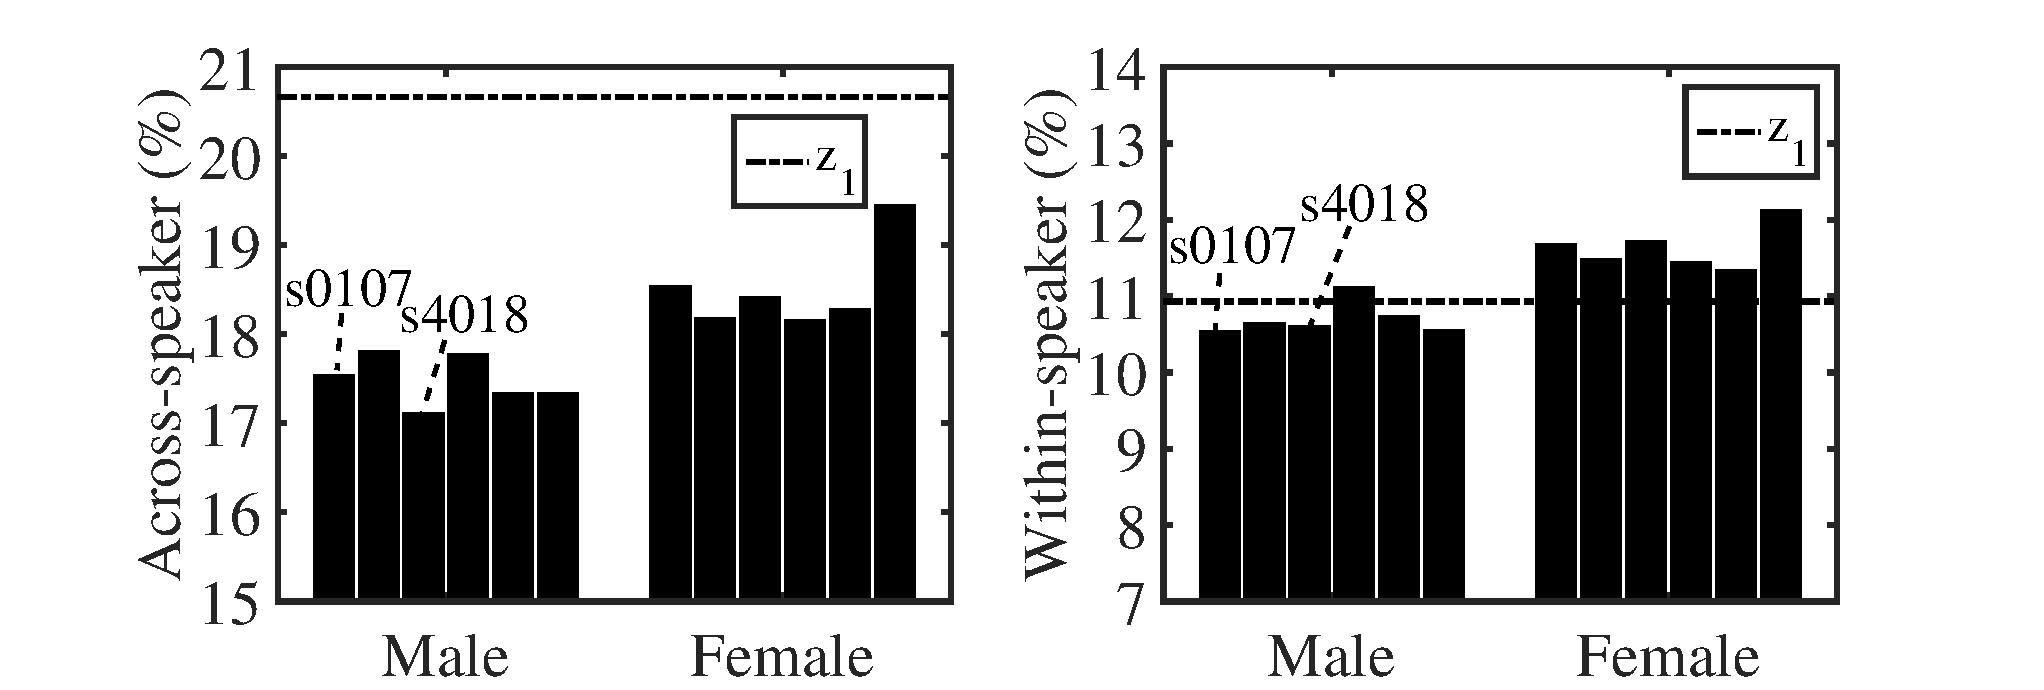
\includegraphics[width=0.9\linewidth]{recon_abx2_export_setup.eps}
    % 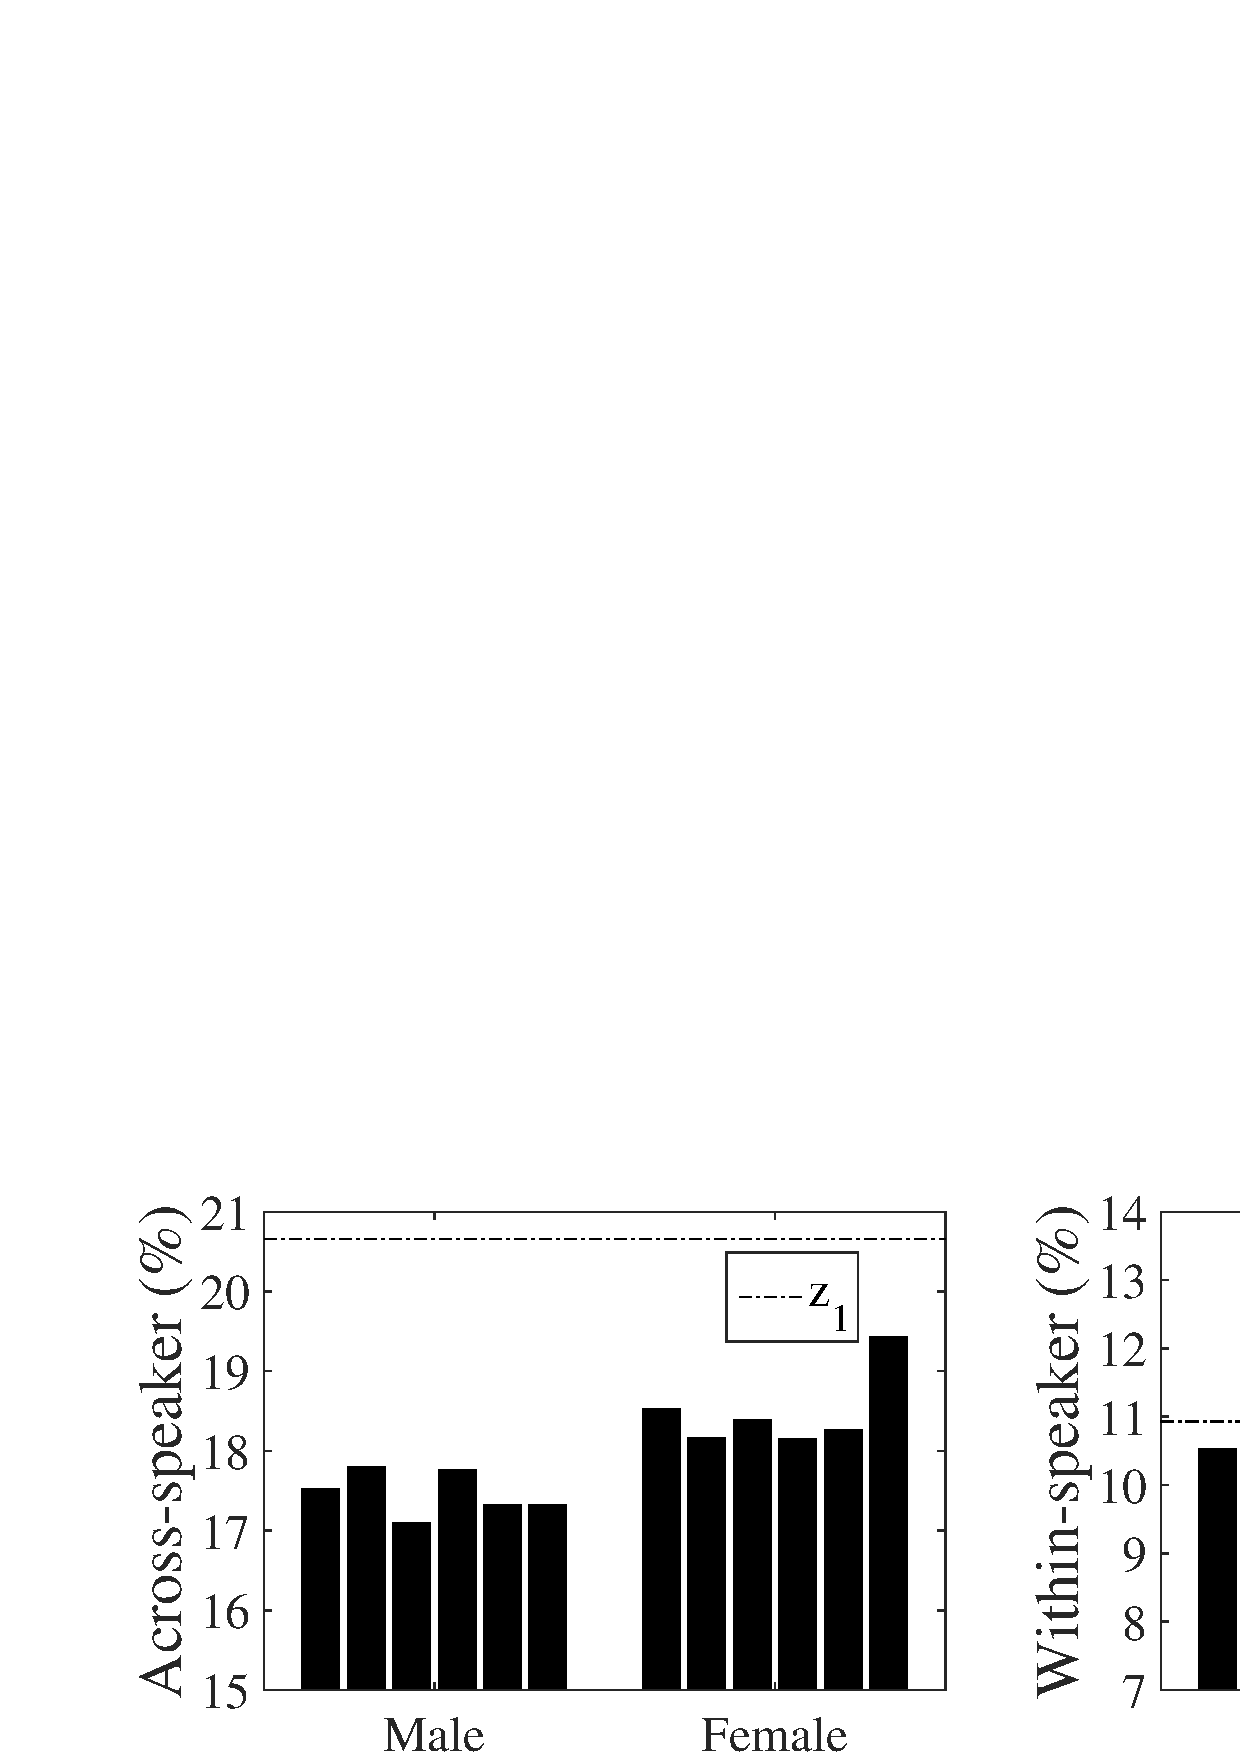
\includegraphics[width=1\linewidth]{recon_abx2.pdf}

    \caption{ABX error rates (\%) on $\bm{\hat{x}}$ using s-vector unification with different representative speakers (Avg. over languages).}
    \label{fig:recon_abx}
\end{figure}
% \subsection{Baseline and systems trained with FHVAE-based speaker-invariant features}
\subsection{DNN-BNFs trained with speaker-invariant features}
Experimental results of the baseline system and systems trained with FHVAE-based speaker-invariant features  are summarized in Table \ref{tab:results}.
The second and third columns of ID $\X1 \sim \X6$ in this Table denote input features to DNN-BNF training and DPGMM clustering, respectively. 
% For example, system \X3 is trained with $\{\bm{z_1}\}$ and its frame labels are generated by clustering $\{\bm{\hat{x}}\}$ with speaker `s0107'.  
`Orig.' denotes original MFCCs without reconstruction, while $\bm{\hat{x}}$-s0107/-s4018 denotes reconstructed MFCCs with representative speaker s0107 or s4018.
% Two male speakers `s4018' and `s0107' are selected as the representative speakers for extracting $\{\bm{\hat{x}}\}$.
% For DPGMM based frame labeling
% In DPGMM clustering, two groups of  reconstructed MFCCs $\{\bm{\hat{x}}\}$ are tested as inputs. One group is corresponding to the representative speaker `s4018', while the other is corresponding to `s0107'. 
Here, $\bm{\hat{x}}$-s4018 is used to  represent the ideal case as it performs the best among the $12$ speakers in across-speaker condition, which is seen in Fig. \ref{fig:recon_abx}.
% ($17.09\%$, $3$-rd  bar from left in Fig. \ref{fig:recon_abx}). 
$\bm{\hat{x}}$-s0107 is used to represent a general case as it performs moderately
% ($17.52\%$, $1$-st bar from left in Fig. \ref{fig:recon_abx}) 
among  the male speakers. 
% In Table \ref{tab:results},
% The second and third columns of ID $\X1 \sim \X6$ denote input features to DNN-BNF training and DPGMM clustering, respectively. 
% % For example, system \X3 is trained with $\{\bm{z_1}\}$ and its frame labels are generated by clustering $\{\bm{\hat{x}}\}$ with speaker `s0107'.  
% `Orig.' means original MFCCs without reconstruction.
% The baseline system in Table \ref{tab:results} does not employ any FHVAE-based speaker-invariant features. 
The system exploiting a  Cantonese ASR for fMLLR estimation \cite{Feng2018exploiting} is denoted as `CA-Sup'. From this Table, several observations are made:

(1) The DNN-BNF models trained with  features $\{\bm{\tilde{x}}\}$ and $\{\bm{z_1}\}$ both outperform that trained with MFCCs. The baseline system and  systems \X1 \& \X2 differ only in DNN-BNF inputs. The results demonstrate the effectiveness in replacing DNN inputs with more speaker-invariant features.
% performing speaker-invariant feature learning towards DNN-BNF inputs.
% BNFs extracted from the DNN model are benefited from the 
% Without improving frame labels, the extracted BNFs can be benefited from 

(2) The reconstructed MFCC features $\{\bm{\hat{x}}\}$ significantly outperform original MFCCs in DPGMM-based frame labeling. 
% In the ideal scenario where the representative speaker is carefully chosen, 
In the ideal case  where the representative speaker `s4018'  is  selected, by comparing \X5 and \X1,  frame labeling based on $\{\bm{\hat{x}}\}$ contributes to  $13.5\%$ and $6.9\%$ relative ABX error rate reductions in across- and within-speaker conditions, compared to that based on original MFCCs. 
% Even 
In a general case where `s0107' is selected, by comparing \X3 and \X1, the relative ABX error rate reductions are  $11.3\%$ and $4.7\%$ in across- and within-speaker conditions.
% respectively. 
The results demonstrate the importance of  frame labeling based on speaker-invariant feature representation.
% employing speaker-invariant features as the input representation for DPGMM clustering.

% They   bring  across-speaker performance improvements  by relative $4.4\%$ and $5.5\%$ respectively. When frame labels are obtained based on reconstructed features with s-vector unification, further improvements are achieved.

(3) Our best system \X5 achieves $2.4\%$ absolute ($17.3\%$ relative) ABX error rate reduction in across-speaker condition, and $0.6\%$ absolute ($7.3\%$ relative) reduction in within-speaker condition, both compared to the baseline DNN-BNF system. 
% The within-speaker error rate reduction is $0.64\%$ absolute and $7.3$ relative. 
Compared to system CA-Sup in which out-of-domain transcribed data are exploited,  \X5 is slightly better in within-speaker condition while slightly inferior in across-speaker condition.  

% is able to close the  topline and baseline across-speaker performance gap by $77\%$. 
% The baseline-topline gap measures the impact of exploiting out-of-domain transcribed speech resources as additional linguistic knowledge in unsupervised subword modeling. With FHVAE-based speaker-invariant learning, $77\%$ of the performance gap can be compensated without requiring any out-of-domain data. 
% Besides, \X5 slightly outperforms topline in within-speaker condition. The relative improvements of \X5 compared to baseline are $17.3\%/7.3\%$ in across-/within-speaker conditions.
% Besides, this system  slightly outperforms the topline system in within-speaker condition. 
% Our best system follows the stricter condition
% It is worth noting that  our best system does not exploit any out-of-domain resources.

We also compare the effectiveness of our proposed approaches with VTLN  reported in \cite{chen2017multilingual}, in which VTLN was adopted to improve frame labels. As seen in Table \ref{tab:results}, in across-speaker  condition, while our baseline system is inferior to their baseline (MFCC), our best system consistently  outperforms their MFCC+VTLN system in all test subsets. 
In within-speaker condition, our proposed approaches also achieve better performance.
% In within-speaker condition, our methods also outperform VTLN. 
The comparison shows that  FHVAE-based speaker-invariant feature learning is more effective than VTLN in improving the quality of frame labels and subword modeling performance.
% learning speaker-invariant features for frame labeling and subword modeling.
% discussed in \cite{Feng2018exploiting} applies a Cantonese ASR for fMLLR estimation.
\section{Conclusions}

This paper presents a study on improving frame labeling for  DNN-BNF unsupervised subword modeling without any out-of-domain resources.
Frame labels are generated by DPGMM clustering towards speaker-invariant features learned from FHVAEs.
% using speaker-invariant features learned from FHVAEs. 
The speaker-invariant features are further fed as inputs to DNN-BNF training.
% The FHVAEs disentangle linguistic content and speaker information encoded in speech in an unsupervised manner. 
% By discarding or unifying speaker information, speaker-invariant features are learned.
% and used as inputs to DNN-BNF frame labeling and model training. 
Experiments conducted on ZeroSpeech 2017 show that our proposed approaches achieve $2.4\%/0.6\%$ absolute  ABX error rate reduction in across-/within-speaker conditions, compared to the baseline without applying FHVAEs.
% are conducted on ZeroSpeech 2017. Experimental results demonstrate the effectiveness of our proposed approaches, especially in across-speaker condition.
Compared with our previous work in which out-of-domain transcribed data are used for speaker adapted feature learning, the approaches in this study are slightly better in within-speaker condition while slightly worse in across-speaker condition.
% The proposed approaches, without requiring any out-of-domain resources, are able to make up $77\%$ of the across-speaker performance gain benefited from exploiting out-of-domain transcribed speech as additional resources.  
Our proposed approaches significantly outperform VTLN in improving the quality of frame labels.

% \section{Acknowledgements}

%  This research is partially supported by a GRF project grant (Ref: CUHK 14227216) from Hong Kong Research Grants Council.

\bibliographystyle{IEEEtran}

\bibliography{mybib}

% \begin{thebibliography}{9}
% \bibitem[1]{Davis80-COP}
%   S.\ B.\ Davis and P.\ Mermelstein,
%   ``Comparison of parametric representation for monosyllabic word recognition in continuously spoken sentences,''
%   \textit{IEEE Transactions on Acoustics, Speech and Signal Processing}, vol.~28, no.~4, pp.~357--366, 1980.
% \bibitem[2]{Rabiner89-ATO}
%   L.\ R.\ Rabiner,
%   ``A tutorial on hidden Markov models and selected applications in speech recognition,''
%   \textit{Proceedings of the IEEE}, vol.~77, no.~2, pp.~257-286, 1989.
% \bibitem[3]{Hastie09-TEO}
%   T.\ Hastie, R.\ Tibshirani, and J.\ Friedman,
%   \textit{The Elements of Statistical Learning -- Data Mining, Inference, and Prediction}.
%   New York: Springer, 2009.
% \bibitem[4]{YourName17-XXX}
%   F.\ Lastname1, F.\ Lastname2, and F.\ Lastname3,
%   ``Title of your INTERSPEECH 2018 publication,''
%   in \textit{Interspeech 2018 -- 19\textsuperscript{th} Annual Conference of the International Speech Communication Association, September 2-6, Hyderabad, India Proceedings, Proceedings}, 2018, pp.~100--104.
% \end{thebibliography}

\end{document}
